\documentclass[12pt,twoside]{scrartcl}
\usepackage[a4paper,top=2cm,left=2cm,right=2cm,bottom=2cm,includefoot,includehead]{geometry}
\usepackage{graphicx}
\usepackage[numbers]{natbib} % Add this line for natbib package
\usepackage{fancyhdr}
\usepackage{hyperref}
\usepackage{amsmath}
\usepackage{circuitikz}
\graphicspath{ {figures/} }


\ctikzset{
    resistor = american,
    % inductor = american,
    voltage = raised ,
    voltage dir = old,
    quadpoles/transformer core/inner = 1, %Eliminates the horizontal bars on the transformer
    quadpoles/transformer core/width = 0.8, %Adjusts the width so that the transformers are closer
    diodes/scale = 0.6,
    capacitors/scale = 0.6,
    resistors/scale = 0.6,
    inductors/scale = 0.8,
    % bipoles/label_distance = 4pt,
    % switch/scale = 0.8,
    % bipoles/length = 1cm,
}

%% shifted open voltage 
\tikzset{open shifted/.style={
    open ,open voltage position=legacy, voltage shift=-0.9}
}

\pagestyle{fancy} % Set the page style to fancy
\fancyhf{} % Clear all header and footer fields

% Define the header and footer content for odd and even pages
\fancyhead[CE,CO]{School of Electrical Engineering} % Left header on even pages, right header on odd pages
% \fancyhead[RE,LO]{Right Header} % Right header on even pages, left header on odd pages
\fancyfoot[LE,RO]{\thepage} % Page number on left footer of even pages and right footer of odd pages
\fancyfoot[RE,LO]{ELEC3251} % Left footer on odd pages, right footer on even pages

\begin{document}
\pagenumbering{arabic}
\setcounter{page}{1}
\begin{titlepage}
    \begin{center}

        \includegraphics[width=0.2\textwidth]{LOGO_Square.pdf}

        \vspace*{0.4cm}
        School of Electrical Engineering \\
        University of Newcastle
        
        \vspace{1cm}
        \huge
        \textbf{\textsf{ELEC3251 \\ Assignment 1}}

        \vspace{0.5cm}
        \large
        \textbf{\textsf{Practical and Theoretical Analysis of \\ Buck Converter and Flyback Converter}}

        \vspace{1.5cm}
        \normalsize
        \begin{tabular}{l|r}
            Liam Patey-Dennis & c3349900 \\
            Joshua Thomas & c3376353
        \end{tabular}
        \vfill    
    \end{center}
\end{titlepage}


\section{Buck Converter}
\subsection{Ideal Calculations}
The duty cycle required to achieve an output voltage of $V_{o} = 5$ V for an input supply voltage of $V_{d} = 12$ V can be determined using the DC transfer function of the Buck converter, see Equation \ref{equation:Buck_TF}. The resulting duty cycle required for the ideal circuit is $D \approx 41.67$\%.\par
\begin{equation}
\frac{V_o}{V_d} = D \label{equation:Buck_TF}
\end{equation}
The output voltage ripple ($\Delta V_o$) of an ideal Buck converter is given by Equation \ref{equation:Buck_ripple}. This equation can be rearranged, see Equation \ref{equation:Buck_cap}, to find the required capacitance for the low pass filter, provided that the duty cycle ($D$), filter inductance ($L$), and switching period ($T_{s}$) are known. For $T_{s} = 1/f_{s} = 10$ $\mu$s, $L = 1$ mH, $D = 41.67$\%, $\Delta V_{o} = 25$ mV, and $V_o = 5$ V, the required capacitance is $C = 1.458$ $\mu$F. \par
\begin{equation}
\frac{\Delta V_{o}}{V_{o}} = \frac{1}{8}\frac{T_{s}^{2}(1-D)}{LC} \label{equation:Buck_ripple}
\end{equation}
\begin{equation}
C = \frac{V_o}{\Delta V_{o}}\frac{T_{s}^{2}(1-D)}{8L} \label{equation:Buck_cap}
\end{equation}
The output power of the converter will be limited by the ratings of the components in the circuit. As the output voltage of the converter is required to remain constant at $5$ V, only the output current can be adjusted to suit the ratings of the components. The inductor selected for the circuit is the Murata \#1410516C, which has a maximum DC current of $1.6$ A \cite{RN1}. A IRFZ24NPbF MOSFET has been selected for the switch, this component has a maximum DC current rating of $17$ A \cite{RN3}. The selected diode is an SB120 which has a maximum DC current of $1.0$ A \cite{RN4}. The inductor current will equal the output current, assuming the voltage across the capacitor remains constant. Therefore, the output current must be less than $1.6$ A, to avoid causing damage to the inductor. The diode will only conduct when the switch is off, therefore the DC current flowing through the diode is $I_{D} = (1-D)I_{o}$. For $I_{o} = 1.6$ A the diode current is $0.93$ A, which is less than the maximum rating of the device. Therefore, the load resistance must be selected such that $I_{o} \le 1.6$ A. Using Ohm’s law this inequality is equivalent to $R_{Load} \ge 3.125$ $\Omega$. The smallest resistor provided in the laboratory kit is $3.9$ $\Omega$ so this resistance will be used for the load.\par
\vspace{5mm}
\noindent The continuous conduction mode (CCM) and discontinuous conduction mode (DCM) boundary occurs when the current flowing through the inductor reaches $0$ A. For the ideal Buck converter this will occur for a DC output current ($I_{oB}$) which can be found using Equation \ref{equation:Buck_DCM}. For the designed converter the minimum DC output current is $I_{oB} = 14.6$ mA, which is equivalent to an output load of $342$ $\Omega$.
\begin{equation}
I_{oB} \approx \frac{T_{s}V_{o}}{2L}(1-D) \label{equation:Buck_DCM}
\end{equation}
\pagebreak
\subsection{Ideal Simulations}
Wolfram System Modeller (Wolfram) was used to simulate the performance of the designed converter. The model used for the simulations is shown in Figure \ref{fig:Buck_idealModel}. The output voltage of the ideal Buck converter is shown in Figure \ref{fig:Buck_idealVout}. The RMS output voltage is 4.9983 V, which lies close to the theoretically expected value of 5 V. The slight discrepancy between the simulated value and the expected value may be the result of truncating the duty cycle to 4 decimal places ($5/12 \approx 0.4167$). It may also be a result of the numerical methods used by the Wolfram software to simulate the system. An output voltage ripple of 6.67 mV is observed. This ripple is smaller than the expected ripple of 25 mV, this may be the result of the assumption that the output ripple is independent of the load impedance. The addition of the load resistance results in an RLC filter at the output of the converter. This resistance dampens the resonant peak of the LC combination which is likely to result in larger amounts of attenuation for the high frequency components of the output voltage.\par
\vspace{5mm}
\noindent Figure \ref{fig:buck_DCM} (A) displays the inductor current for a load resistance of 342 $\Omega$. The current reaches a minimum value of $120 $ $\mu$A, which indicates that the converter is close to the CCM-DCM boundary. Figure \ref{fig:buck_DCM} (b) displays the current for a load resistance of 345 $\Omega$. Slight distortion is observed in the waveform near the zero crossing which indicates that the converter has entered DCM. This suggests that the CCM-DCM boundary lies in the range $342 \le R_{Load} \le 345$ $\Omega$ which agrees with the theoretically expected value of 342 $\Omega$. The boundary may not lie exactly at 342 $\Omega$ because of the assumption, made in Equation \ref{equation:Buck_DCM}, that the inductor current and the output current are equal. This assumption is not correct as a small amount of current also flows through the capacitor.

\begin{figure}[h]
    \centering
    \includegraphics[width=0.7\textwidth]{Buck_idealModel}
    \caption{Modelica model used to simluate the operation of the ideal Buck converter.}
    \label{fig:Buck_idealModel}
\end{figure}

\begin{figure}[h]
    \centering
    \includegraphics[width=0.6\textwidth]{Buck_idealVout}
    \caption{Ideal Buck converter output voltage in steady state. An RMS value of 4.9983 V and a voltage ripple of 6.67 mV are observed.}
    \label{fig:Buck_idealVout}
\end{figure}

\begin{figure}[h!]
    \centering
    \includegraphics[width=0.6\textwidth]{buck_DCM}
    \caption{Buck converter inductor current for a load resistance of (A) 342 $\Omega$, and (B) 345 $\Omega$. A small amount of distortion is present in (B) which indicates that the CCM-DCM boundary lies in the range $342 \le R_{Load} \le 345$ $\Omega$.}
    \label{fig:buck_DCM}
\end{figure}
\newpage

\subsection{Non Ideal Calculations}
The previous calculations and simulations neglect many real-world effects that will affect the circuit's performance. Previously, no voltage losses were assumed to occur across the switch. This assumption is invalid as all switches have non-zero on resistances. Furthermore, it was assumed that no voltage drop occurs across the diode. All diodes have a non-zero voltage drop, which is required to overcome the potential barrier formed at the P-N junction of these devices. In addition, the windings of an inductor are not perfect conductors and hence have resistance. These effects will result in the output voltage of the converter being lower than the theoretically expected value. Applying Kirchoff’s voltage law (KVL) when the switch is on and when the switch is off results in Equations \ref{equation:KVL_on} and \ref{equation:KVL_off}.
\begin{equation}
V_{L,on} = V_{d} - V_{o} - V_{loss, on} = V_{d} - V_{o} - (R_{DS}+ R_{L})i_{L} \label{equation:KVL_on}
\end{equation}
\begin{equation}
V_{L,off} = -V_{o} - V_{f} - V_{loss, off} = V_{o} - V_{f} - R_{L}i_{L}\label{equation:KVL_off}
\end{equation}
Where $R_{DS}$ is the on resistance of the switch, $R_{L}$ is the inductor resistance, and $V_{f}$ is the forward voltage of the diode.\par
\vspace{5mm}
\noindent If it is assumed that the circuit is in steady state, then the zero volt-seconds assumption can be applied which yields,
\begin{equation*}
V_{L,on}t_{on} + V_{L,off}t_{off} = 0
\end{equation*}
If the inductor current is assumed to be equal to the load current then,
\begin{equation*}
i_{L} \approx i_{Load} = \frac{V_{o}}{R_{Load}}
\end{equation*}
Which can be used with the previous equation to obtain Equation \ref{equation:Buck_nonIdealTF}.
\begin{align}
V_{o} &= \frac{R_{Load}}{(1+2D)R_{Load} - R_{L} - DR_{DS}}\left\{DV_{d} - (1-D)V_{f} \label{equation:Buck_nonIdealTF}\right\}
\end{align}
\noindent For the ideal duty cycle ($D = 41.67$\%) with the parameters $R_{DS} = 0.07$ $\Omega$, $R_{L} = 1.6$ $\Omega$, $V_{f} = 0.7$ V and a load current of $i_{L} = 1.28$ A ($R_{Load} = 3.9$ $\Omega$), the expected output voltage of the converter is $V_{o} =3.24$ V \cite{RN1, RN3, RN4}. The duty cycle required to obtain an output of 5 V is $D = 61.44$\%.\par
\vspace{5mm}
\noindent The CCM-DCM boundary occurs when the output current is approximately equal to half of the peak current through the inductor. The peak current through the inductor is given by Equation \ref{equation:buck_iPeak}.\par
\begin{equation}
i_{pk} = \frac{1}{L}\int_{0}^{t_{on}}v_{L} \,dt \label{equation:buck_iPeak}
\end{equation}
\noindent For the ideal case the voltage across the inductor (when the switch is on) is:
\begin{equation*}
v_{L,ideal} = V_{d} - V_{o}
\end{equation*}
For the non-ideal case the voltage is:
\begin{equation*}
v_{L,non-ideal}(t) = V_{d} - V_{o} - i_{L}(t)(R_{DS} + R_{L})
\end{equation*}
Where,
\begin{equation*}
v_{L,ideal} \ge v_{L,non-ideal}(t)
\end{equation*}
Which implies,
\begin{align*}
i_{pk,ideal} &> i_{pk,non-ideal} \\
\intertext{Thus,}
 I_{oB,ideal} &> I_{oB,non-ideal}
\end{align*}
Therefore, it is expected that a larger load resistance will be required for the non-ideal Buck converter, to observe the CCM-DCM boundary.\par

\newpage
\subsection{Non Ideal Simulations}
Figure \ref{fig:Buck_nonIdealModel} displays the Modelica model used to perform the non-ideal simulation. The non ideal switch model from the \textit{InverterParts}.\textit{NonIdeal\_Components} library was used to replicate the IRFZ24NPbF MOSFET. The reverse diode voltage (1.3 V), series resistance (0.07 $\Omega$), parallel resistance (2 M$\Omega$), turn on time (4.9 ns), and turn off time (19 ns) of the MOSFET are included in this model. The 1.6 $\Omega$ resistor is used to model the series resistance of the inductor and the $1.3\times10^{-11}$ F capacitor is used to model the self-resonant frequency of the inductor. The non ideal diode model from the \textit{InverterParts}.\textit{NonIdeal\_Components} library was used to replicate the SB120 diode. The worst case forward voltage (0.70 V) and the junction capacitance (110 pF) of the SB120 were included in this model. An output capacitance of 1 $\mu$F has been used in the simulation. This capacitance was selected as it lies close to the theoretically predicted value and was the largest capacitance that can be achieved with the laboratory kit without placing multiple capacitors in series. \par
\vspace{5mm}
\noindent The output voltage of the non-ideal converter for the ideal duty cycle is shown in Figure \ref{fig:buck_NI_output_oldD}. An RMS voltage of 3.2164 V is observed, which lies close to the theoretically predicted value of 3.24 V. The slight deviation from this value may be the result of assuming that the output current is constant and equal to the current through the inductor. Figure \ref{fig:buck_NI_output_newD} displays the output voltage for a duty cycle of 61.44\%, an RMS voltage of 5.0010 V is observed which lies close the predicted value. A ripple voltage of 27.739 mV is observed which lies close to the specified value of 25 mV. The increase in the voltage ripple for the non-ideal simulation is likely a result of the reducing the size of the output capacitor, increasing the duty cycle, and including the parasitic capacitance of the inductor. This ripple could be reduced through increasing the size of the output capacitor.\par
\begin{figure}[h]
    \centering
    \includegraphics[width=0.7\textwidth]{Buck_nonIdealModel}
    \caption{Modelica model used to simluate the operation of the non ideal Buck converter.}
    \label{fig:Buck_nonIdealModel}
\end{figure}

\begin{figure}[h]
    \centering
    \includegraphics[width=0.6\textwidth]{buck_NI_output_oldD}
    \caption{Non-ideal Buck converter output voltage for duty cycle of 41.67\% and a load of $3.9$ $\Omega$. An average voltage of 3.2164 V is observed.}
    \label{fig:buck_NI_output_oldD}
\end{figure}
\begin{figure}[h]
    \centering
    \includegraphics[width=0.6\textwidth]{buck_NI_output_newD}
    \caption{Non-ideal Buck converter output voltage for duty cycle of 61.44\% and a load of $3.9$ $\Omega$. An average voltage of 5.0010 V and a ripple voltage of 27.739 mV is observed.}
    \label{fig:buck_NI_output_newD}
\end{figure}
\pagebreak

\noindent The current through the inductor for $D = 61.44$\% (rated power conditions) is shown in Figure \ref{fig:buck_Current}. An RMS current of 1.2847 A is observed which matches the theoretically predicted value and does not exceed the maximum ratings of the devices. The inductor current for a load of (A) 470 $\Omega$ and (B) 475 $\Omega$ is shown in Figure \ref{fig:buck_NIDCM}. The inductor current for the 475 $\Omega$ passes through the 0 A crossing for a period of time. This indicates that the circuit has entered DCM. The 470 $\Omega$ load results in a current which gets close to the 0 A crossing. Therefore the load resistance for the CCM-DCM boundary is expected to lie in the range $470 \le R_{Load} \le 475$ $\Omega$. \par
\newpage

\begin{figure}[htp]
    \centering
    \includegraphics[width=0.6\textwidth]{buck_Current.png}
    \caption{Inductor current for the non ideal Buck converter under rated power conditions.}
    \label{fig:buck_Current}
\end{figure}

\begin{figure}[htp]
    \centering
    \includegraphics[width=0.6\textwidth]{buck_NIDCM}
    \caption{Inductor current for the non ideal Buck converter under rated power conditions.}
    \label{fig:buck_NIDCM}
\end{figure}

\subsection{Results}
The constructed Buck converter is shown in Figure \ref{fig:buck_real}. The circuit was constructed on a breadboard and multicore twisted wires were used. The PWM input signal for the gate driver was generated using a signal generator and the output voltage was monitored using an oscilloscope. \par

\begin{figure}[htp]
    \centering
    \includegraphics[width=0.7\textwidth]{buck_real}
    \caption{Constructed Buck converter.}
    \label{fig:buck_real}
\end{figure}

\noindent The observed output voltage of the Buck converter for a duty cycle of $D = 62$\% is shown in Figure \ref{fig:buck_expV_newD}. The blue waveform is the output voltage, and the yellow waveform is the PWM input signal to the gate driver. An RMS output voltage of 5.081 V is observed which lies close to the simulated value of 5.0010 V. A peak to peak voltage of 2.000 V is observed which does not align with the simulated ripple voltage of 27.739 mV. This large peak to peak voltage is a result of the large transients that occur when the PWM signal switches. These transients arise from the parasitic inductances of the wires and the parasitic capacitances of the breadboard. As the PWM signal has infinite bandwidth, some of the components of the signal resonant with the parasitic inductances and capacitances which results in large transient responses that are visible in the output waveform. This ripple can only be mitigated through minimizing the parasitic impedances of the device. This could be achieved through designing a printed circuit board (PCB) for the device. This would reduce the parasitic capacitance of the design, as the capacitance formed by the parallel conductive strips on the breadboard would not be present.  The designed PCB would need to feature short trace lengths with tight ground loops to minimize parasitic inductance.\par
\vspace{5mm}
\noindent To explore the output ripple of the converter once the large transients are no longer present, Figure \ref{fig:buck_expV_ripple} displays the steady state output voltage of the Buck converter for $D = 62$\% . A maximum voltage of 5.14 V and a minimum voltage of 5.02 V is observed which results in an output voltage ripple of 120 mV. This output ripple is much larger than the specified ripple of 25 mV and is larger than the simulated ripple of 27.739 mV.  This is likely due to the parasitic inductances of the wires used. This ripple could be reduced through minimizing the length of the wires and by using a larger output capacitor. A larger output capacitor will result in more attenuation of these high frequency ripple components.\par
\newpage
\begin{figure}[htp]
    \centering
    \includegraphics[width=0.7\textwidth]{buck_expV_newD}
    \caption{Output voltage of the Buck converter (blue) for a duty cycle of 62\%. The yellow waveform is the input PWM signal to the gate driver. An RMS voltage of 5.081 V is observed.}
    \label{fig:buck_expV_newD}
\end{figure}
\begin{figure}[htp]
    \centering
    \includegraphics[width=0.7\textwidth]{buck_expV_ripple}
    \caption{Output voltage of the Buck converter in steady state. A ripple voltage of 120 mV is observed.}
    \label{fig:buck_expV_ripple}
\end{figure}

\noindent Figure \ref{fig:buck_expI} displays the inductor current (green waveform) close to the rated output power conditions ($D = 62$\%). An RMS current of 1.11 A is observed which does not agree with the simulated value of 1.2847 A. This is likely a result of the designed converter not accounting for variation in the resistance of the load. This is evidenced by the RMS output voltage (blue waveform) of 4.75 V which implies the load resistance is 4.27 $\Omega$ instead of 3.90 $\Omega$. This was likely not observed in Figure \ref{fig:buck_expV_newD} as the circuit had been running for a longer period of time when the current was measured, compared to when the voltage was measured. This longer operating period likely resulted in the temperature of the load increasing which leads to a larger number of collisions between the electrons and the ions in the load and hence a larger resistance. The dependence of the output voltage on the load could be removed through the use of a closed loop control system with integral action. \par
\vspace{5mm}
\noindent Figure \ref{fig:buck_expI_DCM} (A) displays the inductor (green waveform) for a load of 470 $\Omega$ and $D = 62$\%. The inductor current is observed to reach 0 A but does not remain there for a considerable amount of time, which indicates that the device is on the cusp of DCM. This result aligns with the simulation results. Figure \ref{fig:buck_expI_DCM} (B) displays the inductor current inductor current (green waveform) and output voltage (blue waveform) for a load resistance of 600 $\Omega$. The current spends a larger amount of time near the zero crossing which indicates that the circuit is in DCM mode.

\begin{figure}[htp]
    \centering
    \includegraphics[width=0.7\textwidth]{buck_expI}
    \caption{Output current of the Buck converter under rated power conditions.}
    \label{fig:buck_expI}
\end{figure}

\begin{figure}[htp]
    \centering
    \includegraphics[width=0.7\textwidth]{buck_expI_DCM}
    \caption{Output current of the Buck converter under rated power conditions.}
    \label{fig:buck_expI_DCM}
\end{figure}
\newpage
\section{Flyback Converter}
\subsection{Ideal Calculations}
\begin{figure}[htp]
    \centering
    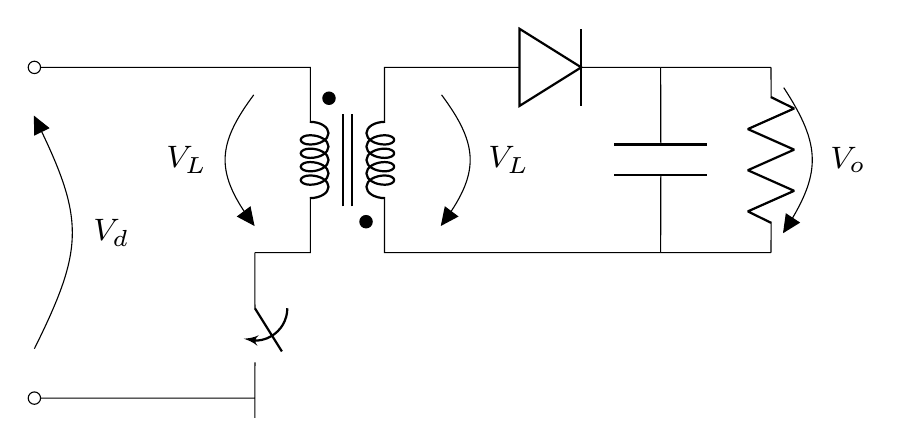
\begin{tikzpicture}[scale=1.4, transform shape]
        % \caption{Ideal Flyback Converter}
        %draw tri and quadpoles
        \node[transformer core, anchor = A1, scale = 0.8](transformer) at (2,2){};
        \node[circ](c1) at (transformer.inner dot A1){};
        \node[circ](c2) at (transformer.inner dot B2){};
        % \node[switch, scale = 0.8](switch1) at (2,0){};
        
        %Primary
        \draw (0,-1)
         to [open,v>=\footnotesize $V_d$,o-o] ++(0,3)
         to (0,2)
         to (2,2)
         to (transformer.A1) % current here
         (transformer.A2) to [switch,transform shape] ++(0,-1.5)
         |- (0,-1);
         
        
        %Secondary
         \draw (transformer.B1) to[Do] ++ (2,0) coordinate(A)
         (A) to[C] (A |- transformer.B2)
         (transformer.B2) to (A |- transformer.B2);
        
         \draw (A) ++(1,0) coordinate(B)
         (A)--(B)
         (B) to [R,v^=\footnotesize $V_o$] (B|- transformer.B2)
         (B|- transformer.B2) -- (A |- transformer.B2);
        
        % \draw (npn.C) to[open shifted, v^=$v_Q$](npn.E);
        % \draw (npn.B) to[open shifted, v=$v_{be}$, voltage shift=-1](npn.E);
        \draw (transformer.A1) to[open shifted, v=\footnotesize $V_L$](transformer.A2);
        \draw (transformer.B1) to[open shifted, v^>=\footnotesize$V_L$](transformer.B2);
        
        
        \end{tikzpicture}
        \label{tikzpicture:idealFlyback}
        \caption{Ideal Flyback Converter}
    \end{figure}
    \noindent
    To determine the required duty cycle for the ideal flyback converter, the zero volt seconds rule is applied. 
    It is assumes that no losses occur at the transformer, switches and diodes. In this instance, it is also assumed that the transformer turns ratio is 1:1.
    For the case in which the switch is closed, 
    \begin{equation}
        V_d - V_L = 0
    \end{equation}
    The secondary side has no influence, as the inductor is assumed to be in steady state. 
    For the case where the switch is open,
    \begin{equation}
        -V_L - V_o = 0
    \end{equation}
    The application of the zero-volts second rule,
    \begin{equation}
        DT_s \cdot V_{L \: on} + (1-D)T_s \cdot V_{L\:off} = 0
        \label{equation:zerovoltseconds}
    \end{equation}
    Cancel out $T_s$, then substitute equations $V_L$ equations,
    \begin{equation}
        D \cdot V_d+ (1-D) \cdot -V_o = 0
    \end{equation}
    Therefore, the duty cycle becomes,
    \begin{equation}
        D  = \dfrac{V_o}{V_d+V_o}
    \end{equation}
    The design specifications desire $V_o$ to be 10V but specifys 
    the input, $V_d$, to be a range of [5,12]V.
    For $V_{d\:max}$, 
    \begin{equation}
        D = \dfrac{10}{12+10} = 45.45\:\%
    \end{equation}
    and for 
    $V_{d\:min}$,
    \begin{equation}
        D = \dfrac{10}{5+10} = 66.67\:\%
    \end{equation}
    For the ideal flyback converter, the load resistance can be calculated 
    from the desired output power and desired output voltage,
    \begin{equation}
        R_L = \dfrac{V_o^2}{P_o}
    \end{equation}
    Therefore, if $V_o$ = 10 V and $P_o$ = 0.5 W then $R_L = 200\: \Omega $. 
    To ensure CCM and a reasonable voltage ripple, the output capacitor, C, 
    is calculated from the voltage ripple equation for the flyback, the same equation as the buck-boost converter.
    \begin{equation}
        \Delta V_o = \dfrac{DT_s}{CR_L}V_o
        \label{equation:voltageRipple}
    \end{equation}
    If the switching frequency is 100 kHz, then $T_s$ = 10 $\mu$s. Then rearranging to make C the subject and substituting relevant parameters,
    \begin{equation}
        C = \dfrac{DT_s}{\Delta V_oR_L}V_o 
        % = \dfrac{0.4545 \cdot 10 \mu}{0.2 \cdot 200}10
        \label{equation:capacitance}
    \end{equation}
    Hence, for $V_{d\:max}$, $C$ = 1.136 $\mu$F and for $V_{d\:min}$, $C$ = 1.56 $\mu$F
\newpage
\subsection{Ideal Simulations}

\begin{figure}[htp]
    \centering
    \includegraphics[width=0.75\textwidth]{ModellicaIdeal.PNG}
    \caption{Ideal Flyback, Output Voltage $V_o$ = 10 V, ($V_d$ = 12 V, $D$ = 0.4545)}
    \label{fig:IdealModellica}
\end{figure}

\newpage

\begin{figure}[htp]
    \centering
    \includegraphics[width=0.75\textwidth]{IdealSim12V.png}
    \caption{Ideal Flyback, Output Voltage $V_o$ = 10 V, ($V_d$ = 12 V, $D$ = 0.4545)}
    \label{fig:IdealSim12V}
\end{figure}

\begin{figure}[htp]
    \centering
    \includegraphics[width=0.75\textwidth]{PowerIdealSim12V.png}
    \caption{Ideal Flyback, Output Power $P_o$ = 0.5 W, ($V_d$ = 12 V, $D$ = 0.4545)}
    \label{fig:PowerIdealSim12V}
\end{figure}

\begin{figure}[htp]
    \centering
    \includegraphics[width=0.75\textwidth]{RippleIdealSim12V.png}
    \caption{Ideal Flyback, Output Ripple $\Delta V_o$ = 200 mV, ($C$ = 1 $\mu$F, $V_d$ = 12 V, $D$ = 0.4545)}
    \label{fig:RippleIdealSim12V}
\end{figure}
% All simulations met expectations. 
\begin{figure}[htp]
    \centering
    \includegraphics[width=0.75\textwidth]{IdealSim5V.png}
    \caption{Ideal Flyback, Output Voltage $V_o$ = 10 V, ($V_d$ = 5 V, $D$ = 0.6667)}
    \label{fig:IdealSim5V}
\end{figure}

\begin{figure}[htp]
    \centering
    \includegraphics[width=0.75\textwidth]{PowerIdealSim12V.png}
    \caption{Ideal Flyback, Output Power $P_o$ = 0.5 W, ($V_d$ = 5 V, $D$ = 0.6667)}
    \label{fig:PowerIdealSim5V}
\end{figure}

\begin{figure}[htp]
    \centering
    \includegraphics[width=0.75\textwidth]{RippleIdealSim5V.png}
    \caption{Ideal Flyback, Output Ripple $\Delta V_o$ = 300 mV, ($C$ = 1 $\mu$F, $V_d$ = 5 V, $D$ = 0.6667)}
    \label{fig:RippleIdealSim5V}
\end{figure}


\newpage
\subsection{Non-Ideal Calculations}
\begin{figure}[htp]
    \centering
    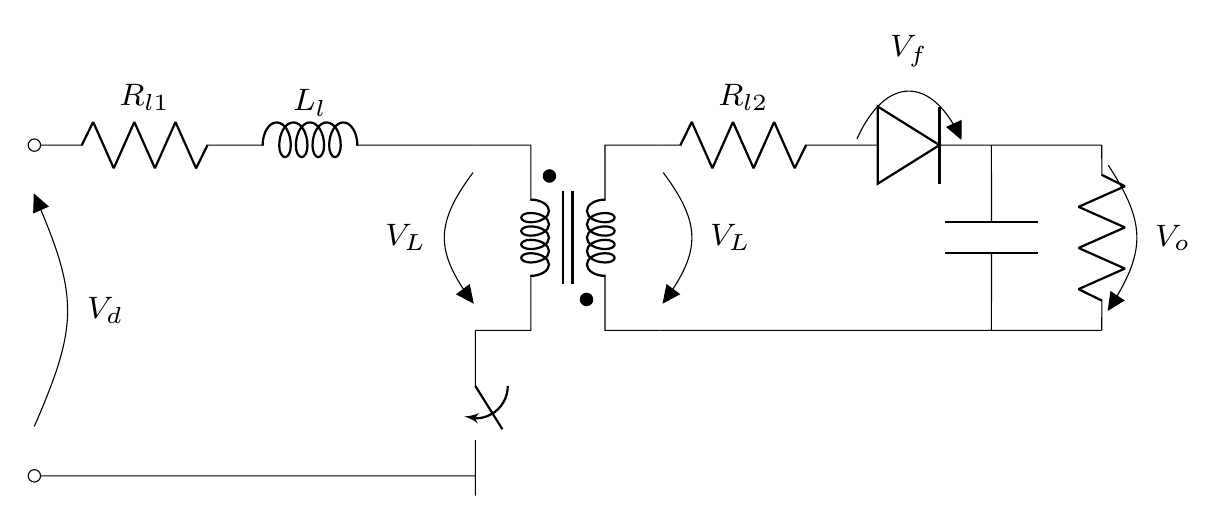
\begin{tikzpicture}[scale=1.4, transform shape,voltage shift=-0.5]
        % \caption{Ideal Flyback Converter}
        %draw tri and quadpoles
        \node[transformer core, anchor = A1, scale = 0.8](transformer) at (2,2){};
        \node[circ](c1) at (transformer.inner dot A1){};
        \node[circ](c2) at (transformer.inner dot B2){};
        % \node[switch, scale = 0.8](switch1) at (2,0){};
        
        %Primary
        \draw (-2,-1)
         to [open,v>=\footnotesize $V_d$,o-o] ++(0,3)
         to (-2,2)
         to [R,l^=\footnotesize $R_{l1}$,label distance = 2pt] (0,2)
         to [L,l^=\footnotesize $L_{l}$] (1,2)
         to (transformer.A1) % current here
         (transformer.A2) to [switch,transform shape] ++(0,-1.5)
         |- (-2,-1);
         
        
        %Secondary
         \draw (transformer.B1)
        %  to [L,l^=\footnotesize $L_{l2}$] ++(1.5,0)
         to [R,l^=\footnotesize $R_{l2}$,label distance = 2pt] ++(1.5,0)
         to [Do,v^=\footnotesize $V_f$] ++(1.5,0) coordinate(A)
         (A) to [C] (A |- transformer.B2)
         (transformer.B2) to (A |- transformer.B2);
        
         \draw (A) ++(1,0) coordinate(B)
         (A)--(B)
         (B) to [R,v^=\footnotesize $V_o$] (B|- transformer.B2)
         (B|- transformer.B2) -- (A |- transformer.B2);
        
        % \draw (npn.C) to[open shifted, v^=$v_Q$](npn.E);
        % \draw (npn.B) to[open shifted, v=$v_{be}$, voltage shift=-1](npn.E);
        \draw (transformer.A1) to[open shifted, v=\footnotesize $V_L$,voltage shift=-0.8](transformer.A2);
        \draw (transformer.B1) to[open shifted, v^>=\footnotesize$V_L$,voltage shift=-0.8](transformer.B2);
        
        
        \end{tikzpicture}
        \label{tikzpicture:nonidealFlyback}
        \caption{Non-Ideal Flyback Converter}
    \end{figure}
    \noindent The specifications for the flyback converter ask for an output of 10 V at 0.5 W. 
    To achieve this, an average current can be calculated using ohm's law of power,
    \begin{equation}
        P = IV
    \end{equation}
    which gives $I_{avg}$ = 50 mA. This can be used to determine the load resistance with ohm's law,
    \begin{equation}
        V = IR
        \label{equation:ohm}
    \end{equation}
    Therefore, the load resistance, $R_L$ is $200\: \Omega$. The closest available load resistor is $220\: \Omega$ which can be reversed to get the average current,
    $I_{avg}$ = 45.45 mA and output power, $P = 0.4545$ W which is now the standard and will be used for further calculations.
    The non-ideal components of the current flyback converter can be 
    modelled like this. The primary side is the only active when the 
    switch is on, this means the internal MOSFET resistance and the internal 
    transformer resistance can be added together like this,
    \begin{equation}
        R_{l1} = R_{mosfet} + R_{transformer}
        \label{equation:Rp}
    \end{equation}
    For the case when switch is closed,
    \begin{equation}
        V_d - V_{Rl1} - V_{Ll} - V_L = 0
    \end{equation}
    The voltage across the leakage inductance cannot be known, instead the 
    leakage inductance will be ratioed in terms of the magnetising inductance. From the transformer datasheet, \cite{RN2}, the magnetising 
    inductance is $3$ mH and the leakage inductance at the primary side is $9\:\mu$H. Therefore the case when
    the switch is closed is simplified to,
    \begin{equation}
        V_d - V_{Rl1} - V_L = 0
    \end{equation}
    Therefore the case for the switch is open,
    \begin{equation}
        -\dfrac{3}{3.009}V_L - V_{Rl2} - V_f - V_o = 0
    \end{equation}
    Applying the zero volt seconds rule, \ref{equation:zerovoltseconds}, and cancelling out Ts,
    \begin{equation}
        D \cdot( V_d - V_{Rl1} ) + (1-D) \cdot \dfrac{3.009}{3}(- V_{Rl2} - V_f - V_o) = 0
    \end{equation}
    rearranging to make duty cycle the subject,
    \begin{equation}
        D  = \frac{\dfrac{3.009}{3}(V_{Rl2} + V_f + V_o)}{V_d - V_{Rl1} + \dfrac{3.009}{3}(V_{Rl2} + V_f + V_o)}
    \end{equation}
    Equation \ref{equation:Rp}, is used to calculate $R_{l1} = 1.47$. 
    It is known that the average current, $I_{avg} = 45.45$ mA, \ref{equation:ohm}. The duty cycle can 
    be calculated for the maximum and minimum of the desired $V_d$ range [5,12]V. For $V_{d\:max}$,
    \begin{equation}
        D  = \frac{\dfrac{3.009}{3}(1.7\cdot I_{avg} + 0.7 + 10)}{12 - 1.47\cdot I_{avg} + \dfrac{3.009}{3}(1.7\cdot I_{avg} + 0.7 + 10)} = 47.53\: \%
    \end{equation}
    and for $V_d\:min$,
    \begin{equation}
        D  = \frac{\dfrac{3.009}{3}(1.7\cdot I_{avg} + 0.7 + 10)}{5 - 1.47\cdot I_{avg} + \dfrac{3.009}{3}(1.7\cdot I_{avg} + 0.7 + 10)} = 68.66\: \%
    \end{equation}

\newpage

\subsection{Non-Ideal Simulations}

\begin{figure}[htp]
    \centering
    \includegraphics[width=0.75\textwidth]{ModellicaNonIdeal.PNG}
    \caption{Non Ideal Flyback, Output Voltage $V_o$ = 9.21 V, ($V_d$ = 5 V, $D$ = 0.6667)}
    \label{fig:NonIdealModellica}
\end{figure}
\noindent
In all non-ideal simulations, the capacitance is set to 1 $\mu$F. This is less than what was calculated, \ref{equation:capacitance}, and it should be noted.

\newpage
\begin{figure}[htp]
    \centering
    \includegraphics[width=0.75\textwidth]{NonIdealSim12V(calculated).png}
    \caption{Non Ideal Flyback, Output Voltage $V_o$ = 9.746 V, ($V_d$ = 12 V, $D$ = 0.4753)}
    \label{fig:NonIdealSim12Vcal}
\end{figure}

\begin{figure}[htp]
    \centering
    \includegraphics[width=0.75\textwidth]{NonIdealSim12V(tested).png}
    \caption{Non Ideal Flyback, Output Voltage $V_o$ = 10 V, ($V_d$ = 12 V, $D$ = 0.4815)}
    \label{fig:NonIdealSim12Vtested}
\end{figure}

\begin{figure}[htp]
    \centering
    \includegraphics[width=0.75\textwidth]{PowerNonIdealSim12V.png}
    \caption{Non Ideal Flyback, Output Power $P_o$ = 0.432 W, ($V_d$ = 12 V, $D$ = 0.4753)}
    \label{fig:PowerNonIdealSim12V}
\end{figure}

\begin{figure}[htp]
    \centering
    \includegraphics[width=0.75\textwidth]{RippleNonIdealSim12V.png}
    \caption{Non Ideal Flyback, Output Ripple $\Delta V_o$ = 210 mV, ($V_d$ = 12 V, $D$ = 0.4753)}
    \label{fig:RippleNonIdealSim12V}
\end{figure}
% All simulations met expectations. 
\begin{figure}[htp]
    \centering
    \includegraphics[width=0.75\textwidth]{NonIdealSim5V(calculated).png}
    \caption{Non Ideal Flyback, Output Voltage $V_o$ = 9.21 V, ($V_d$ = 5 V, $D$ = 0.6866)}
    \label{fig:NonIdealSim5Vcal}
\end{figure}

\begin{figure}[htp]
    \centering
    \includegraphics[width=0.75\textwidth]{NonIdealSim5V(tested).png}
    \caption{Non Ideal Flyback, Output Voltage $V_o$ = 10.02 V, ($V_d$ = 5 V, $D$ = 0.7055)}
    \label{fig:NonIdealSim5Vtested}
\end{figure}

\begin{figure}[htp]
    \centering
    \includegraphics[width=0.75\textwidth]{PowerNonIdealSim12V.png}
    \caption{Non Ideal Flyback, Output Power $P_o$ = 0.385 W, ($V_d$ = 5 V, $D$ = 0.6667)}
    \label{fig:PowerNonIdealSim5V}
\end{figure}

\begin{figure}[htp]
    \centering
    \includegraphics[width=0.75\textwidth]{RippleNonIdealSim5V.png}
    \caption{Non Ideal Flyback, Output Ripple $\Delta V_o$ = 290 mV, ($V_d$ = 5 V, $D$ = 0.6667)}
    \label{fig:RippleNonIdealSim5V}
\end{figure}
\newpage

\subsection{Results}

\begin{figure}[htp]
    \centering
    \includegraphics[width=0.7\textwidth]{Flyback_Built.jpg}
    \caption{Practical Flyback, $C$ = 2.68 $\mu$F}
    \label{fig:Practical}
\end{figure}

\begin{table}[h!]
    \centering
    \caption{Comparison of Duty Cycles ($D$) required to produce $V_o$ = 10 V}
    \begin{tabular}{c|c c}
    $V_d$ & 12V & 5V \\
    \hline
    Calculated $D$ & 0.4753 & 0.6866 \\
    
    Simulated $D$ & 0.4815 & 0.7055 \\
    
    Practical $D$ & 0.491 & 0.734 \\
    
    \end{tabular}
    
    \label{tab:duty_cycle}
    \end{table}
    

\newpage

\begin{figure}[htp]
    \centering
    \includegraphics[width=0.7\textwidth]{Flyback/tek0001.png}
    \caption{Practical Flyback, Ripple $\Delta V_o$ = 344 mV, ($C$ = 1 $\mu$F, $V_d$ = 12 V, $D$ = 0.477)}
    \label{fig:Practical1}
\end{figure}

\begin{figure}[htp]
    \centering
    \includegraphics[width=0.7\textwidth]{Flyback/tek0002.png}
    \caption{Practical Flyback, Ripple $\Delta V_o$ = 128 mV, ($C$ = 2.68 $\mu$F, $V_d$ = 12 V, $D$ = 0.477)}
    \label{fig:Practical2}
\end{figure}

\begin{figure}[htp]
    \centering
    \includegraphics[width=0.7\textwidth]{Flyback/tek0003.png}
    \caption{Practical Flyback, Output Voltage $V_o$ = 8.32 V, ($C$ = 2.68 $\mu$F, $V_d$ = 5 V, $D$ = 0.688)}
    \label{fig:Practical3}
\end{figure}

\begin{figure}[htp]
    \centering
    \includegraphics[width=0.7\textwidth]{Flyback/tek0004.png}
    \caption{Practical Flyback, Output Voltage $V_o$ = 10 V, ($C$ = 2.68 $\mu$F, $V_d$ = 5 V, $D$ = 0.734)}
    \label{fig:Practical4}
\end{figure}

\newpage
\subsection{Conclusion}
The flyback was successfully built and could meet all specifications 
including the input voltage range, $V_d$ = [5,12]V. 
Some non-ideal behaviour and theory differences was observed. 
These include the practical procedure to meet specifications, the gate-driver noise and the mistake with the
non-ideal transformer model which will be discussed. 
\\\\
The built flyback needed to be adjusted to meet specifications. To reduce the voltage ripple \ref{fig:Practical1}, the capacitance was increased 
from 1 $\mu$F to 2.68 $\mu$F by placing capacitors in parallel \ref{fig:Practical}, which is known to reduce
the output voltage ripple from \ref{equation:voltageRipple}. This is 
expected to create an output ripple of 76 mV. Implementing this greatly reduces the output voltage ripple from 344 mV to 128 mV, 
\ref{fig:Practical2}. While it does not match the expected $\Delta V_o$, it does match the linear 
relationship between capacitance and voltage ripple. The output voltage did not match the desired 
specification, $V_o$ = 10 V, \ref{fig:Practical3}. To fix this, the duty cycle was increased
until output voltage specification was met, see \ref{fig:Practical4}. This increased the duty cycle,
from 0.688 to 0.734 and does not meet theory expectations. 
\\\\
The output voltage noise was much greater in the buck converter. This is seen by comparing the buck converter peak-peak measurement, figure \ref{fig:buck_expI_DCM}
to the flyback converter peak-peak measurement, \ref{fig:Practical1}.  
This is because when the gate driver was used it was plugged into a breadboard, \ref{fig:Practical} which creates 20 pF between the pins on each side. This is amplified 
by switching harmonics, similar to bipolar vs unipolar. In the buck converter,
the gate driver must drive the gate of the MOSFET to a greater voltage because it is set up in the high side configuration. 
In the flyback converter, the MOSFET is setup in a low side configuration, which means the gate voltage doesn't require more than 5 V logic high.
\\\\
The transformer calculations did not correctly model the simulation and practical behaviour. From the theory in equation \ref{equation:zerovoltseconds}, a ratio was used 
to determine power lost at the primary. This however does not accurately reflect lost power, which increases with a higher duty cycle. 
This relationship is viewed by comparing figure (\ref{fig:NonIdealSim12Vcal}, \ref{fig:NonIdealSim12Vtested}) to (\ref{fig:NonIdealSim5Vcal}, \ref{fig:NonIdealSim5Vtested}) and considering Table \ref{tab:duty_cycle}.
This occurs because the average current at the primary side will increase with respect to the duty cycle. A better relationship would be to use the voltage inductor law,
\begin{equation}
    V_{Ll} = L \dfrac{di}{dt}
\end{equation} 
which can be converted to discrete time,
\begin{equation}
    V_{Ll} = L_l \dfrac{\Delta I_p}{T_s}
    \label{equation:discreteInductor}
\end{equation}
It is assumed that the power is conserved across transformer,
\begin{equation}
    V_pI_p = V_sI_s
\end{equation}
therefore the change in current at the primary side is estimated by considering the voltage ripple.
\begin{equation}
    \Delta I_p = \dfrac{V_s}{V_p} \cdot \dfrac{\Delta V_o}{R_L}
\end{equation} 
Therefore, the average voltage drop across the leakage inductance 
can be calculated from the inductor relationship, \ref{equation:discreteInductor}. Then, 
$V_{Ll}$ = 3.27 mV for $V_d$ = 5 V and $V_{Ll}$ = 1.36 mV for $V_d$ = 12 V. The transformer current rule
can also be used to adjust the voltage drop across the primary side internal resistance. This would more accurately 
reflect the power losses due to the transformer as the calculations will be using the primary side current to 
determine voltage drops. Latex Report


\newpage
\bibliographystyle{IEEEtranN}
\bibliography{references}

\end{document}
